\subsection{Introduction}
In order to spoof the onboard GPS, the CAN-bus was chosen as input to AQ. 
The CAN-bus is already implemented and widely used on a ViaCopter drone to communicate between AQ and hardware like ESCs, PDB etc. Much time was spend reading through the source code and trying to figure out how the protocol works.
The developers behind AQ says, that the code is the documentation and thereby have not written any real documentation. \\
Figuring out how it works was done using debugging utilities such as breakpoints and looking at the content of the different memory locations in CrossWorks.
To further investigate the protocol a PEAK-CAN adapter were connected to a Ladybird drone and several python scripts were developed to send and receive messages from AQ. \\
The author did not go into details about messages used between AQ $\leftrightarrow$ ESC's and AQ $\leftrightarrow$ OSD.\\


\subsection{CAN Protocol description}
A Peak-CAN adapter were used throughout the project. It supports High-speed ISO 11898-2\footnote{\url{http://www.peak-system.com/PCAN-USB.199.0.html?&L=1}} which is a standard that states the properties of physical layer. 
Its max speed is 1 mbit which is the speed AQ uses to communicate on the CAN-bus. 
AQ uses CAN 2.0B which has 29 identifier bits.
AQ is not using an existing protocol on top of ISO 11898-2. The developers created their own to suit their needs.\\

\subsubsection{Identifier bits}
A Generic look at a AQ CAN messages can be seen in table \ref{tab:can_identifier_bits}.
The normal function of the identifier bits is the priority of the messages.
A CAN controller can then be setup to only allow certain messages to be processed depending on their identifier bits.
The identification bits has been split up in AQ to contain information about the sender, receiver etc. Which is not normally saved information in a CAN message.
\begin{table}[H]
\resizebox{\textwidth}{!}{%
	\begin{tabular}{|c|c|c|c|c|c|c|c|}
	\hline
	\multicolumn{8}{|c|}{CAN Message} \\ 
	\hline
	 \multicolumn{7}{|c|}{Identfier bits [29 bits]} &  		\multicolumn{1}{c|}{Data bits [max 64 bits]} \\
	 \hline
	 LCC [28:27] & TT [26] & FID [25:22] & DOC [21:16] & SOID 	[15:11] & TID [10:16] & SEID [5:0] & \\
	\hline
\end{tabular}}
	\caption{Table shows the identifier bits used in AutoQuad CAN messages}
	\label{tab:can_identifier_bits}
\end{table}

In figure \ref{tab:abbri_can_msg} the abbreviations can be seen.
\begin{table}[H]
		\begin{tabular}{|l|l|}
		\hline
		LCC & Logical Communications Channe \\
\hline
		TT & Target Type \\
\hline
		FID & Function ID \\
\hline
		DOC & Data Object Code \\
\hline
		SOID & Source ID \\
\hline
		TID & Target ID \\
\hline
		SEID & Sequence ID \\
\hline
		\end{tabular}
		\caption{Table shows 
abbreviations used in table \ref{tab:can_identifier_bits}}
		\label{tab:abbri_can_msg}
\end{table}

Each of the elements in an AQ messages will be explained how they are used in AQ. \\

\subsubsection{Logic Communication Channel}
LCC is the priority of the message. 
To understand how LCC works, one needs to look into CAN arbitration.
As stated in ISO-11898-2, a 0 is the dominant bit and a 1 is the recessive bit.
The example in figure \ref{tab:can_arbitration} shows two nodes each transmitting a packet.
The arbitration only happens during the transmission of the identifier bits.
In the example on bit 8, Node 16 losses the arbitration and stops transmitting.
Node 15 keeps transmitting its packet because it has lower identifier bits and thereby higher priority.
\begin{figure}[H]
    \center
    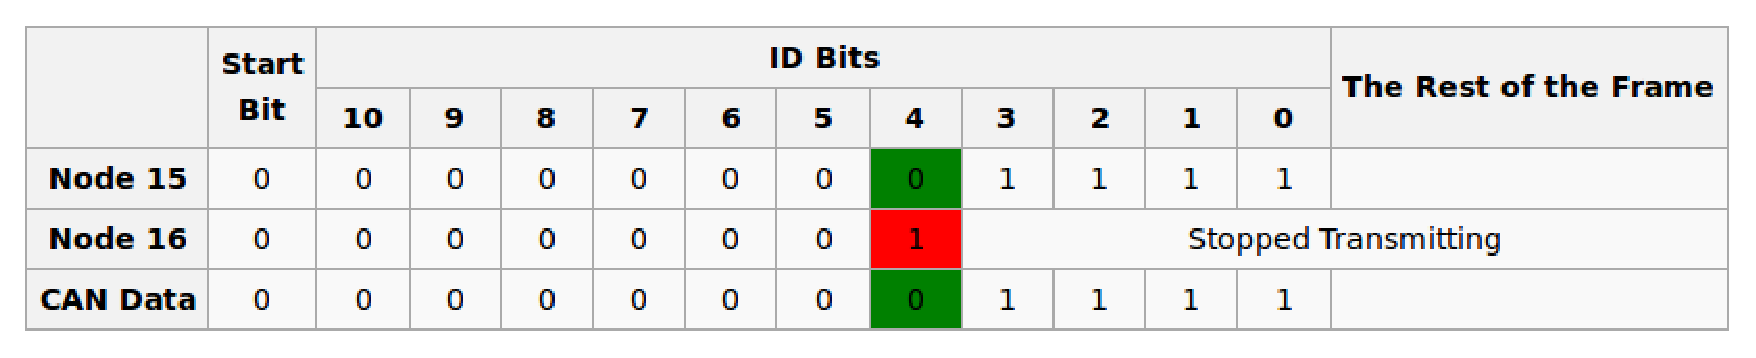
\includegraphics[width=1\textwidth]{graphics/can_arbitration.eps}
    \caption{Example of CAN arbitration where node 15 has the lowest ID and thereby highest priority}
    \label{tab:can_arbitration}
\end{figure}
\newpage
LLC in a message can take one of the defines in code \ref{code:llc_defines}
\begin{lstlisting}[language = c, caption = LLC defines, label=code:llc_defines]
#define CAN_LCC_EXCEPTION   ((uint32_t)0x0<<30)
#define CAN_LCC_HIGH        ((uint32_t)0x1<<30)
#define CAN_LCC_NORMAL      ((uint32_t)0x2<<30)
#define CAN_LCC_INFO        ((uint32_t)0x3<<30)
\end{lstlisting}

\begin{table}[H]
\centering
\caption{Table showing the 4 types of priority in AQ}
\label{my-label}
\begin{tabular}{|l|l|l|}
\hline
\textbf{Name} & \textbf{Value} & \textbf{Priority (lowest first)} \\ \hline
EXCEPTION     & 0000           & 0                 \\ \hline
HIGH          & 0001           & 1                 \\ \hline
NORMAL        & 0010           & 2                 \\ \hline
INFO          & 0011           & 3                 \\ \hline
\end{tabular}
\end{table}

\subsubsection{Target Type}
Target type can either be “node” or “group” depending on if the receiver(s) is one or more nodes. 
\begin{lstlisting}[language = c, caption = Target type defined in AQ, label=code:target_types]
#define CAN_TT_GROUP        ((uint32_t)0x0<<29)
#define CAN_TT_NODE         ((uint32_t)0x1<<29)
\end{lstlisting}
The GROUP is used when AQ sends its reset-msg upon startup.\\
When the authors node send a sensor-measure to AQ it will be of type NODE.
\subsubsection{Function ID}

Function ID describes the function of the CAN message. If it is a PING, ACK, NACK, etc.
It simply states the function of packet so the receiver node knows what to do with the message.
Different types of functions can be seen in code \ref{code:function_defines}
\begin{lstlisting}[language = c, caption = Excerpts from AQ's list of function defines, label=code:function_defines]
#define CAN_FID_RESET_BUS		((uint32_t)0x0<<25)
#define CAN_FID_ACK				((uint32_t)0x1<<25)
#define CAN_FID_REQ_ADDR		((uint32_t)0x7<<25)
#define CAN_FID_GRANT_ADDR	((uint32_t)0x8<<25)
\end{lstlisting}

Table \ref{tab:fid_descriptions} describes the FIDs shown in code \ref{code:function_defines}.
\begin{table}[H]
\centering
\caption{Descriptions of the FIDs mentioned in code \ref{code:function_defines}}
\label{tab:fid_descriptions}
\resizebox{\textwidth}{!}{%
\begin{tabular}{|l|l|}
\hline
\textbf{FID}          & \textbf{Description}                                                               \\ \hline
CAN\_FID\_RESET\_BUS  & Message sent by AQ when powered up                                                 \\ \hline
CAN\_FID\_ACK         & Message sent to AQ when acknowledging a received message                           \\ \hline
CAN\_FID\_REQ\_ADDR   & Messaged used when a node on the bus tries to register itself as a node in AQ \\ \hline
CAN\_FID\_GRANT\_ADDR & Messaged sent by AQ when it registers a node on the bus.                 \\ \hline
\end{tabular}
}
\end{table}
\subsubsection{Data Object Code}
Comming.. Kind of parameter to FID
\Mathias{eksempel på hvordan de bliver brugt i koden - vise function id i switch/case}
\Mathias{Dscripe how the node is created on the BUS}

\subsubsection{Source/Target/Network ID}
When referred to source/target ID but without respect to either sender or receiver but just a CAN-node, then it is referred to as NetworkId.

\subsubsection{Sequence ID}
The sequence id is incremented on transmission of each message. It is used when eg. 
A CAN-node sends a reply to a get-message, it is then including the sequence id of the get-message so AQ knows what it receives a reply for.

\subsubsection{Data bits}
The data bytes does not have a general definition, it depends on the function id.

When FID is CAN\_FID\_REQ\_ADDR, data has the following information in data byte[] and [] respectively.
\begin{itemize}
	\item Uuid
	\item Can type
\end{itemize}

\subsection{Registering a node in AQ}
\begin{sequencediagram}
  \newthread{0.4}{pynode}{ROS-node}
  \newthread{7}{autoquad}{AutoQuad}

  \mess{autoquad}{RESET}{pynode}

  \begin{call}[3]{autoquad}{Wait(100ms)}{autoquad}
		\postlevel
		\postlevel
		\mess{pynode}{REQADDR}{autoquad}
		\postlevel
		\mess{autoquad}{GRANTADDR}{pynode}
  \end{call}
  \mess{autoquad}{CanTelemeryValue}{pynode}
  \mess{pynode}{ACKValue*}{autoquad}
  \postlevel

  \mess{autoquad}{CanTelemetryRate}{pynode}
  \mess{pynode}{ACKRate}{autoquad}
\end{sequencediagram}

Test of sending sensor data
\begin{figure}[H]
    \center
    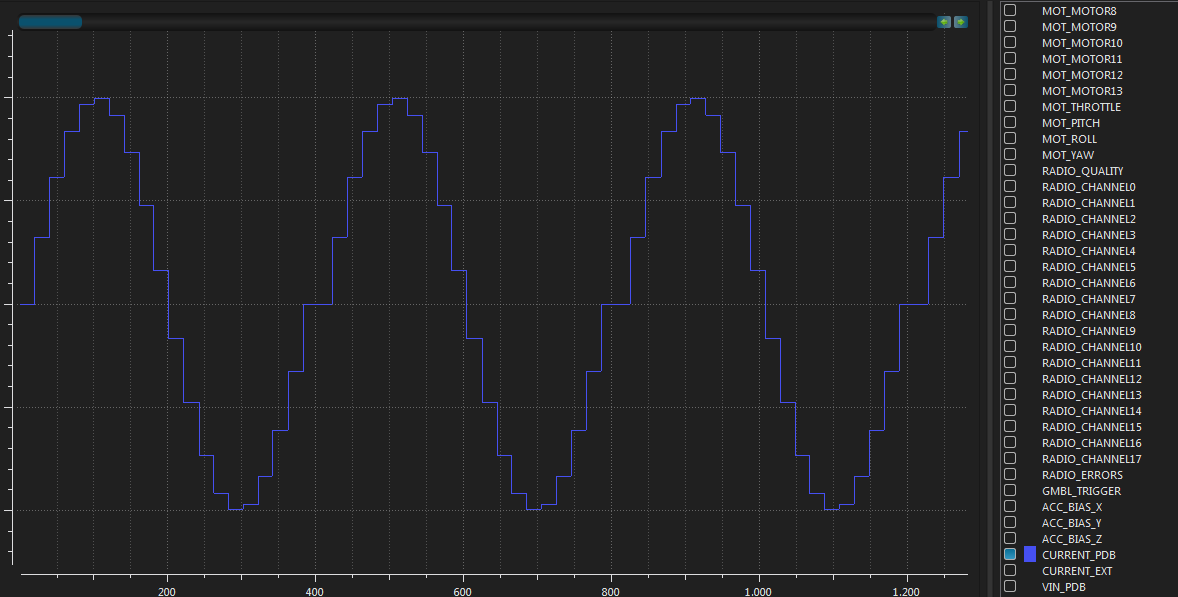
\includegraphics[width=0.8\textwidth]{graphics/test_can_spoof_current.png}
    \caption{Test of python CAN test}
    \label{fig:PCB_block}
\end{figure}